\section{Ajustes al trabajo terminal}
En esta sección se definen todas las nuevas estrategias a seguir para agilizar y 
optimizar el desarrollo del juego.

\subsection{Correción del enfoque de la solución}
Para el enfoque de solución se decide remplazar la gamificación por el termino 
\textit{Serious Games}. Esta modificación nace a partir de la pregunta de: 
“¿Se puede gamificar un videojuego?”. Definiendo la gamificación como el uso de 
elementos del juego y el pensamiento basado en juego en entornos no relacionados 
con el juego para aumentar el compromiso o modificar el comportamiento
\cite{RefIntroGamificacion}, la gamificación de un juego resulta en una contradicción 
del mismo concepto ya que gamificación solo es aplicable a entornos ajenos a 
juegos. Por su parte \textit{Serious Games} queda definido como juegos cuyo 
propósito va más allá del entrenamiento\cite{Ref:Serious}. Los 
\textit{Serious Games} pueden ser utilizados para la educación, la capacitación, 
la medicina como medio terapéutico y en última instancia para la persuasión, es 
decir un juego puede hacer cociente al jugador de algún problema 
\cite{ferreira2002serious}. El concepto de \textit{Serious Games} se ajusta 
al enfoque que aborda el juego desarrollado durante el presente trabajo terminal. 
Esta modificación no impacta directamente en el trabajo que se tenía hasta el 
punto en el que se cambia el enfoque de la solución; siendo esta modificación 
un cambio en el empleo de un tecnicismo para hablar sobre el proyecto.


\subsection{Nueva división de trabajo} \label{Sec:AsignacionTrabajo}
Para realizar la segunda parte del trabajo terminal se decidió cambiar la división 
del trabajo con el objetivo de agilizar el desarrollo. Al terminar los sprints 
anteriores se podía observar que la realización de un nivel estaba llevando 
demasiado tiempo. Por tal motivo se decide reorganizar la asignación de 
tareas, en lugar de que los miembros del equipo de desarrollo se encarguen del 
mismo nivel, se reparten los niveles restantes del desarrollo entre los 
integrantes del equipo. Quedando la asignación de los niveles como se ve en la 
figura \ref{fig:Tareas} .

		\begin{figure}[h]
    			\centering
    			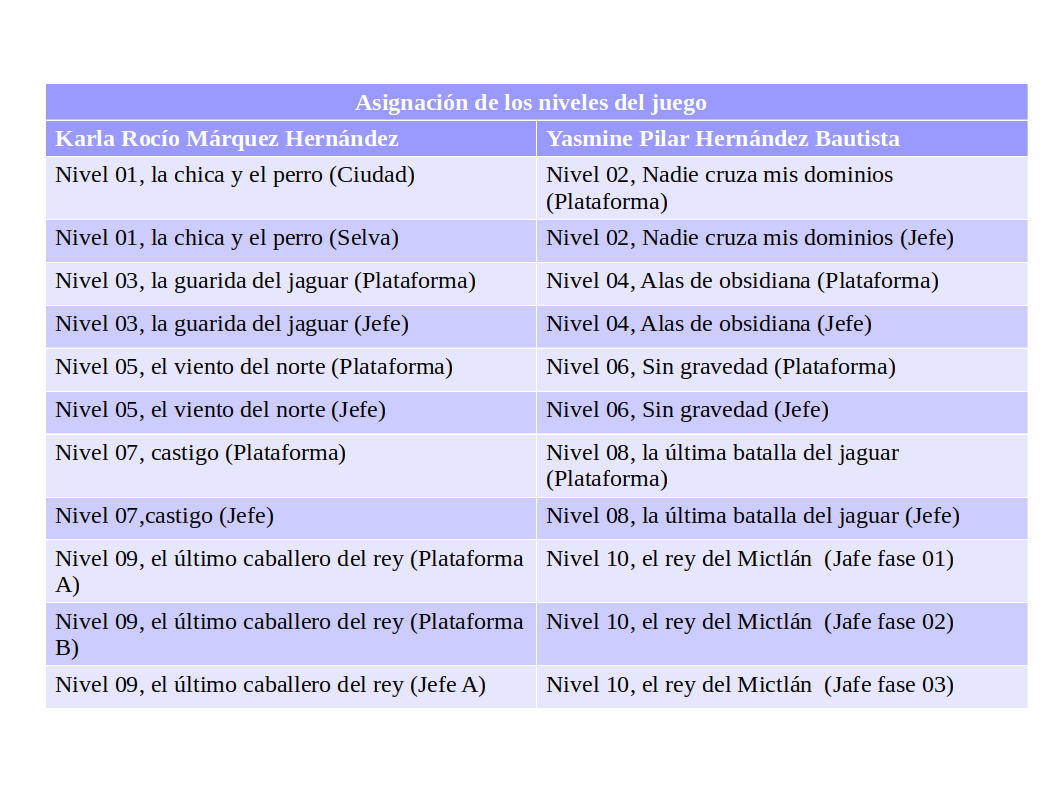
\includegraphics[width=0.8\textwidth]{02Antecedentes/Imagenes/tareasAsignacion.png}
    			\caption{Asignacion de tareas}
    			\label{fig:Tareas}
		\end{figure}


Esta división de trabajo permite que los niveles se desarrollen de manera 
paralela y no de manera secuencial como se había trabajado hasta este \textit{sprint}; 
simulando de esta forma un flujo de trabajo similar a procesamiento multihilo, en 
el que cada integrante del equipo es un hilo y desarrolla sus tareas de manera paralela 
al otro.

\subsection{Actualizando el motor de juego}
Se decidió cambiar la versión 5.4 de \textit{Unity} por la version versión 
2017.3.1f de \textit{Unity3D}. Esta versión incluye herramientas que agilizan la 
creación de niveles como el uso de: 
	\begin{itemize}
		\item \textbf{\textit{Tilemap}:} Herramienta para el mapeado de niveles. Esta 
		herramienta facilita la creación de mapas al crear una malla sobre la que 
		se arrastraran diferentes \textit{Sprites} que se hayan importado previamente 
		al tilemap (ver figura \ref{fig:TilemapPantalla}). En la sección 
		\ref{ConstruccionNivel} se profundizará su funcionamiento.
		
		\begin{figure}[h]
    			\centering
    			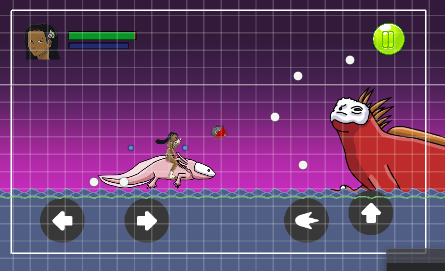
\includegraphics[width=0.6\textwidth]{02Antecedentes/Imagenes/tilemaps01.png}
    			\caption{Vista de la escena cuando se tiene un \textit{GameObject} de 
    			tipo \textit{Tilemaps} para la construcción de niveles}
    			\label{fig:TilemapPantalla}
		\end{figure}
		
		\item \textbf{\textit{Cinemachine}:} \textit{Asset} que permite controlar la 
		cámara de la escena, con este \textit{asset} se le puede indicar que objeto se 
		desea que la cámara siga y se puede asignar un área que limitara el movimiento 
		de la cámara (ver figura \ref{fig:CinemaPantalla}). \textit{Cinemachine} se 
		descarga directamente desde la tienda de \textit{assets} de \textit{Unity} y 
		fue desarrollado por los ingenieros de \textit{Unity}, lo que significa que 
		no genera conflictos o no requiere de configuraciones extras al proyecto para 
		importar. En la sección \ref{Cinemachine} se profundizará su funcionamiento.
			
			\begin{figure}[h]
    			\centering
    			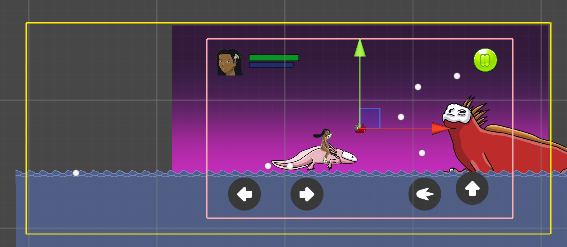
\includegraphics[width=0.6\textwidth]{02Antecedentes/Imagenes/cinemachine01.png}
    			\caption{Vista de la escena cuando se tiene un \textit{GameObject} de 
    			tipo \textit{Tilemaps} para la construcción de niveles}
    			\label{fig:CinemaPantalla}
			\end{figure}

		\item \textbf{\textit{Sprite Packer}}: Si bien no es una herramienta para 
		construcción de niveles o un \textit{asset}, esta herramienta es una de las 
		más útiles que se agregó a la nueva versión de \textit{Unity} ya que, como 
		su nombre lo indica, permite el empaquetado de \textit{sprites} (ver figura 
		\ref{fig:TilemapPantalla}). Empaquetar 
		los \textit{sprites} es una práctica que optimiza el renderizado de objetos, 
		ya que el controlador de gráficos de \textit{Unity} realiza una sola llamada 
		por paquete cuando renderiza los objetos y con esa única llamada renderiza todos 
		los objetos de la escena que se encuentren en ese paquete; si los 
		\textit{sprites} no se encontraran dentro de un paquete el controlador de 
		gráficos de \textit{Unity} haría una llamada por cada \textit{sprite}.  
			\begin{figure}[h]
    			\centering
    			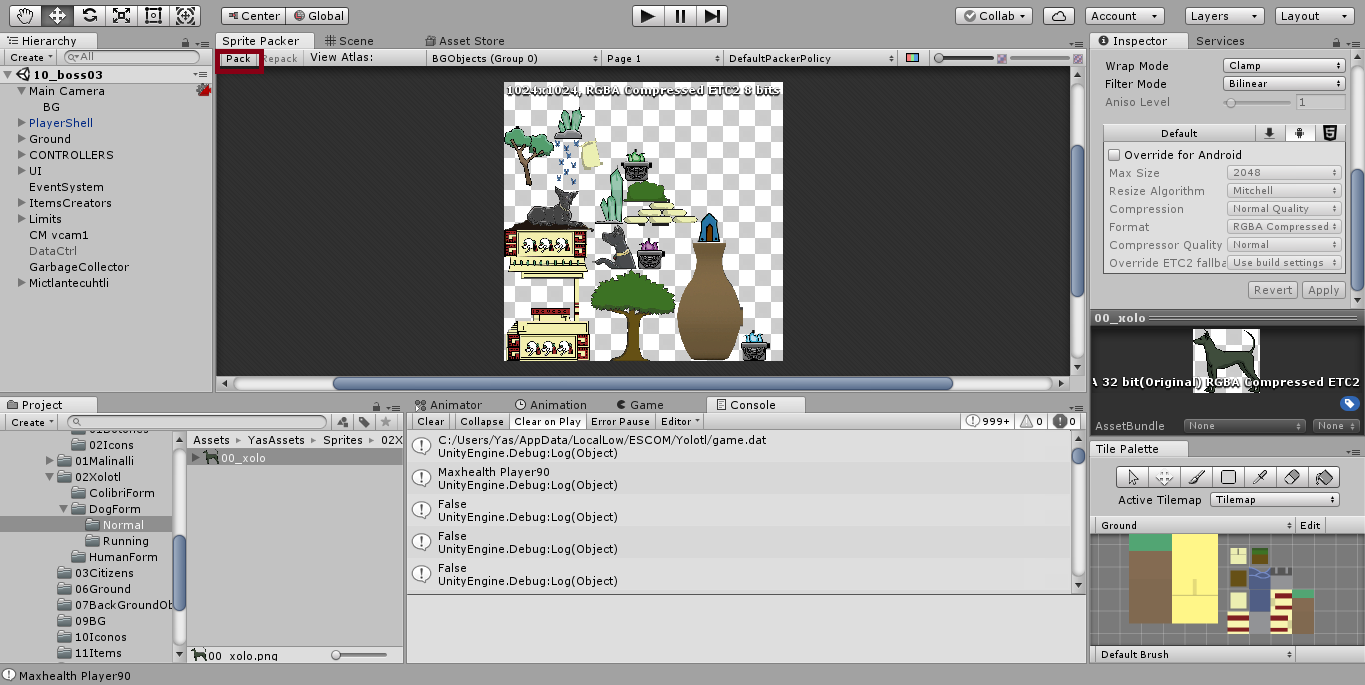
\includegraphics[width=0.6\textwidth]{02Antecedentes/Imagenes/01.png}
    			\caption{Vista de la pestaña del \textit{Sprite Packer}.}
    			\label{fig:CinemaPantalla}
			\end{figure}
	\end{itemize}
	Por el impacto que tendrían las nuevas herramientas de la versión de 
	\textit{Unity}, se propusó utilizarla en lugar de la versión 5.6.2f1. Antes 
	de actualizar la versión de \textit{Unity} se investigó si el proyecto sufriría 
	algún impacto negativo como falta de compatibilidad de componentes por la 
	diferencia de versiones. Al comprobar que existía una total compatibilidad 
	entre ambas versiones en cuanto a trasladar un proyecto de la versión 5.6.1f 
	a la versión 2017.3.1f. Se determinó que la nueva versión de \textit{Unity} 
	sería la que se emplearía para el resto del desarrollo del juego.
	

\section{Máquina de estados}\label{maquinaEdos}
Para las acciones del jefe en los niveles 3, 5, 7 y 9 se utiliza un autómata finito. El estado final es "Morir", donde este representa la destrucción del objeto. 
	\\[1pt]
	
\subsubsection{Jefe nivel 3}
Dada las acciones descritas anteriormente en el documento de diseño, se tiene coraza, impacto, lluvida de rocas, rugido. Además se agregan otras acciones no contempladas para la ayuda de transiciones.
La nomenclatura queda como sigue:
	\\[1pt]
	
\begin{itemize}
	\item Morir -> Mo
	\item Coraza -> Co
	\item Impacto -> Im
	\item Correr x4 -> Cx4
	\item Correr x1 -> Cx1
	\item Rugido -> RA
	\item Lluvia de rocas -> LR
	\item Vida 0 -> V0
	\item Esperar 2 seg. -> E2s
	\item Esperar 1 seg. -> E1s
	\item Jugador cerca -> Jc
\end{itemize}
	\\[1pt]

Los estados son:
	\\[1pt]
	Q = {Mo, Co, Im, Cx4, Cx1, RA, LR}
		\\[1pt]
		
El alfabeto son:
	\\[1pt]
	\sigma = {Jl, V0, E2s, E1s, Jc}
		\\[1pt]
		
El estado inicio es:
	\\[1pt]
	q0 = {LR}
		\\[1pt]
		
El estado final es:
	\\[1pt]
	F = {Mo}
		\\[1pt]

Como vemos en la imagen \ref{fig:maqN3} queda representada la máquina de estados.
\begin{figure}
	\centering
	\caption{Máquina de estados que realiza el jefe del nivel 3}
	\label{fig:maqN3}
	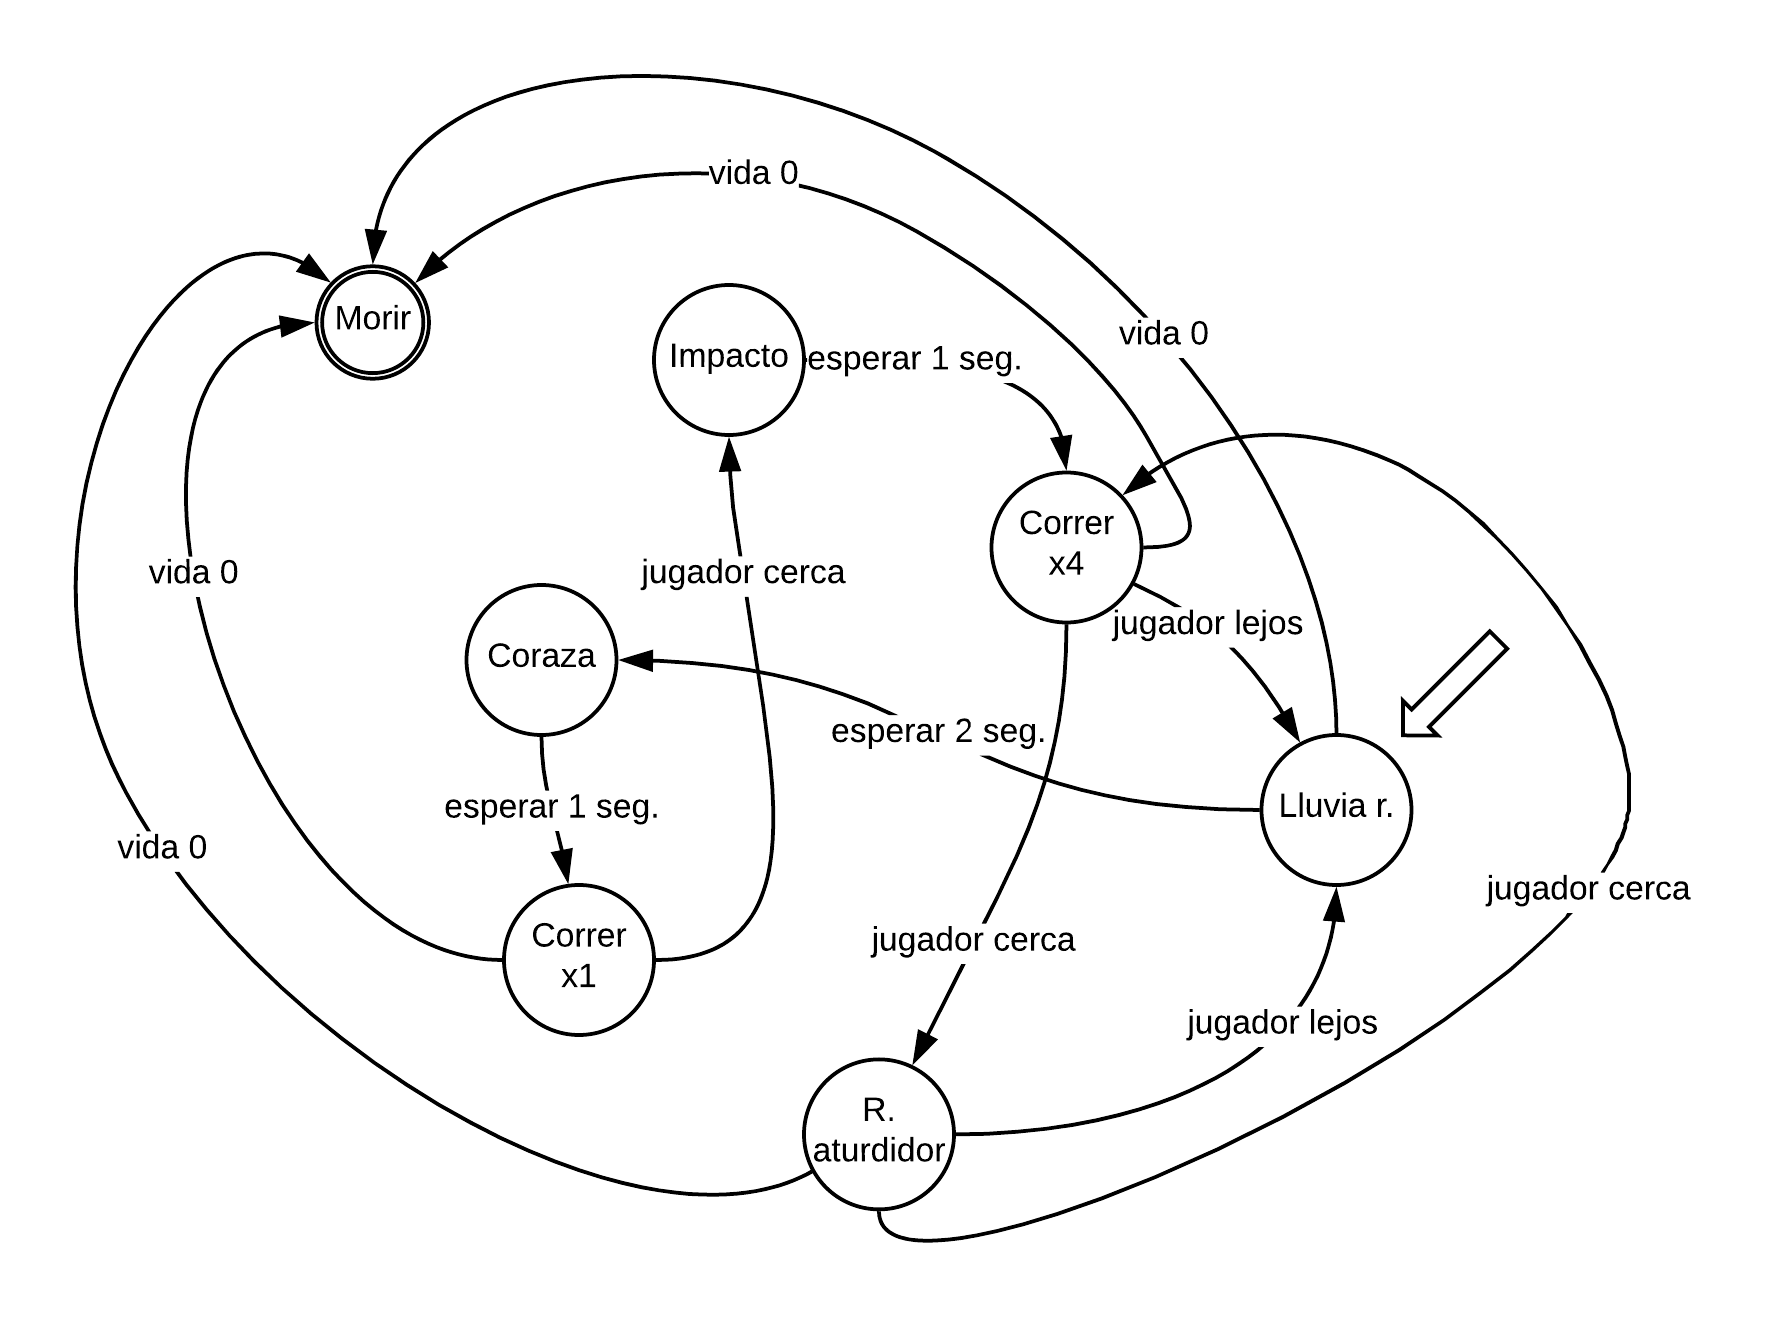
\includegraphics[width=0.5\textwidth]{imagenes\N3}
\end{figure}

\subsubsection{Jefe nivel 5}
Dada las acciones descritas anteriormente en el documento de diseño, se tiene ventisca y tornado. Además se agregan otras acciones no contempladas para la ayuda de transiciones.
La nomenclatura queda como sigue:
\\[1pt]

\begin{itemize}
	\item Morir -> Mo
	\item Estático x4 -> Ex4
	\item Estático x2 -> Ex2
	\item Tornado -> To
	\item Ventisca -> Ve
	\item Vida 0 -> V0
	\item Jugador lejos -> Jl
	\item Esperar 1 seg. -> E1s
	\item Jugador cerca -> Jc
\end{itemize}
\\[1pt]

Los estados son:
\\[1pt]
Q = {Mo, Ex4, Ex2, To, Ve}
\\[1pt]

El alfabeto son:
\\[1pt]
\sigma = {Jl, V0, E1s, Jc}
\\[1pt]

El estado inicio es:
\\[1pt]
q0 = {Ex4}
\\[1pt]

El estado final es:
\\[1pt]
F = {Mo}
\\[1pt]

Como vemos en la imagen \ref{fig:maqN5} queda representada la máquina de estados.

\begin{figure}
	\centering
	\caption{Máquina de estados que realiza el jefe del nivel 5}
	\label{fig:maqN5}
	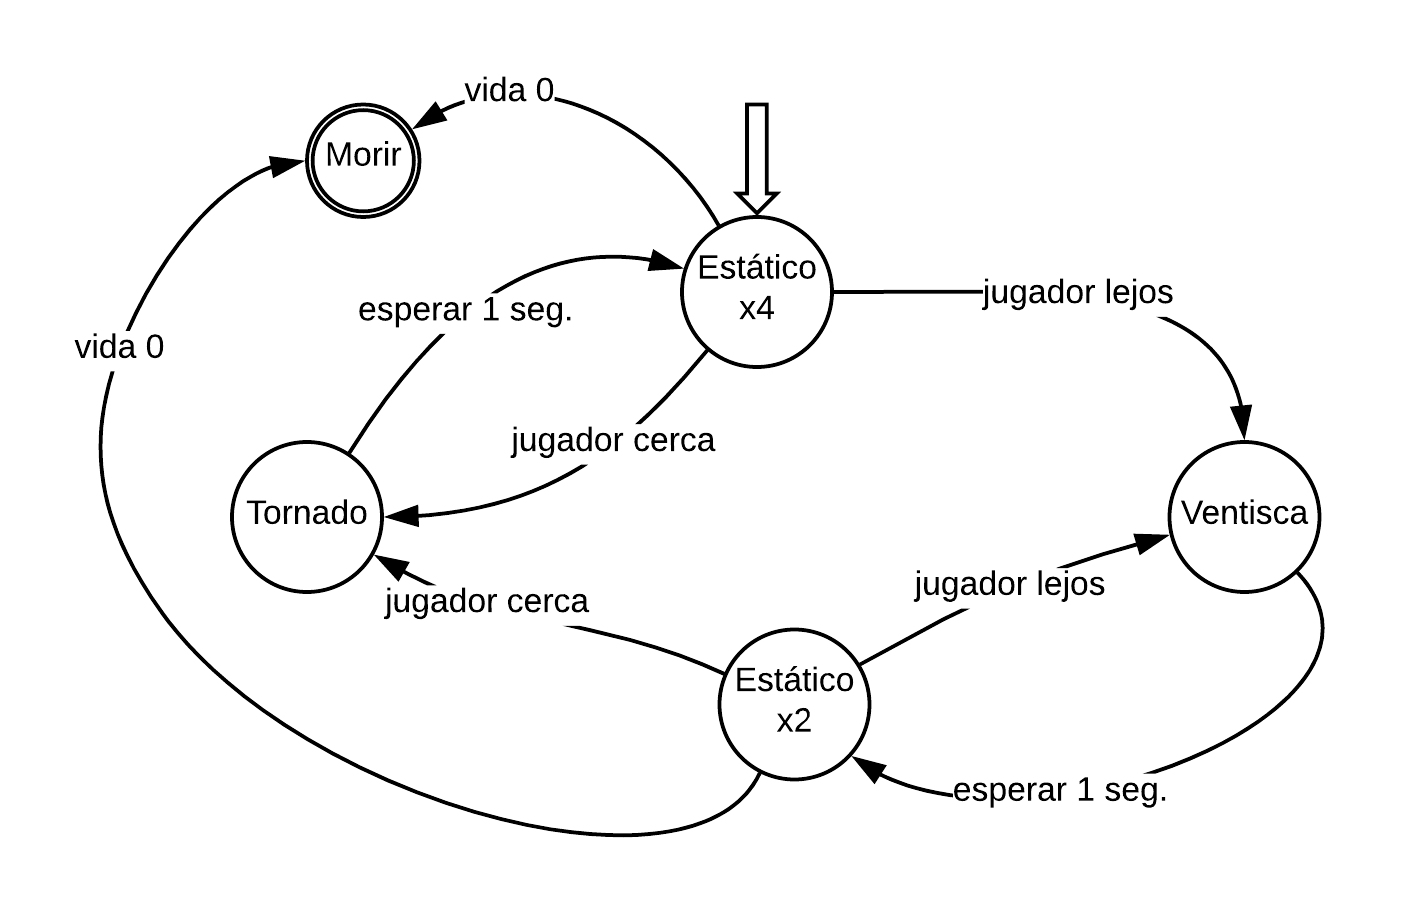
\includegraphics[width=0.5\textwidth]{imagenes\N5}
\end{figure}

\subsubsection{Jefe nivel 7}
Dada las acciones descritas anteriormente en el documento de diseño, se tiene lluvia de flechas, manotazo, lava. Además se agregan otras acciones no contempladas para la ayuda de transiciones.
La nomenclatura queda como sigue:
\\[1pt]

\begin{itemize}
	\item Morir -> Mo
	\item Estático x4 -> Ex4
	\item Estático x3 -> Ex3
	\item Estático x2 -> Ex2
	\item Manotazo -> Ma
	\item Lava -> La
	\item Lluvia flechas -> Lf
	\item Vida 0 -> V0
	\item Rand 0 -> R0
	\item Rand 1 -> R1
	\item Rand 2 -> R2
\end{itemize}
\\[1pt]

Los estados son:
\\[1pt]
Q = {Mo, Ex4, Ex2, Ex3, Ma, La, Lf}
\\[1pt]

El alfabeto son:
\\[1pt]
\sigma = {V0, R0, R1, R2}
\\[1pt]

El estado inicio es:
\\[1pt]
q0 = {Ex3}
\\[1pt]

El estado final es:
\\[1pt]
F = {Mo}
\\[1pt]


Como vemos en la imagen \ref{fig:maqN7} queda representada la máquina de estados.

\begin{figure}
	\centering
	\caption{Máquina de estados que realiza el jefe del nivel 7}
	\label{fig:maqN7}
	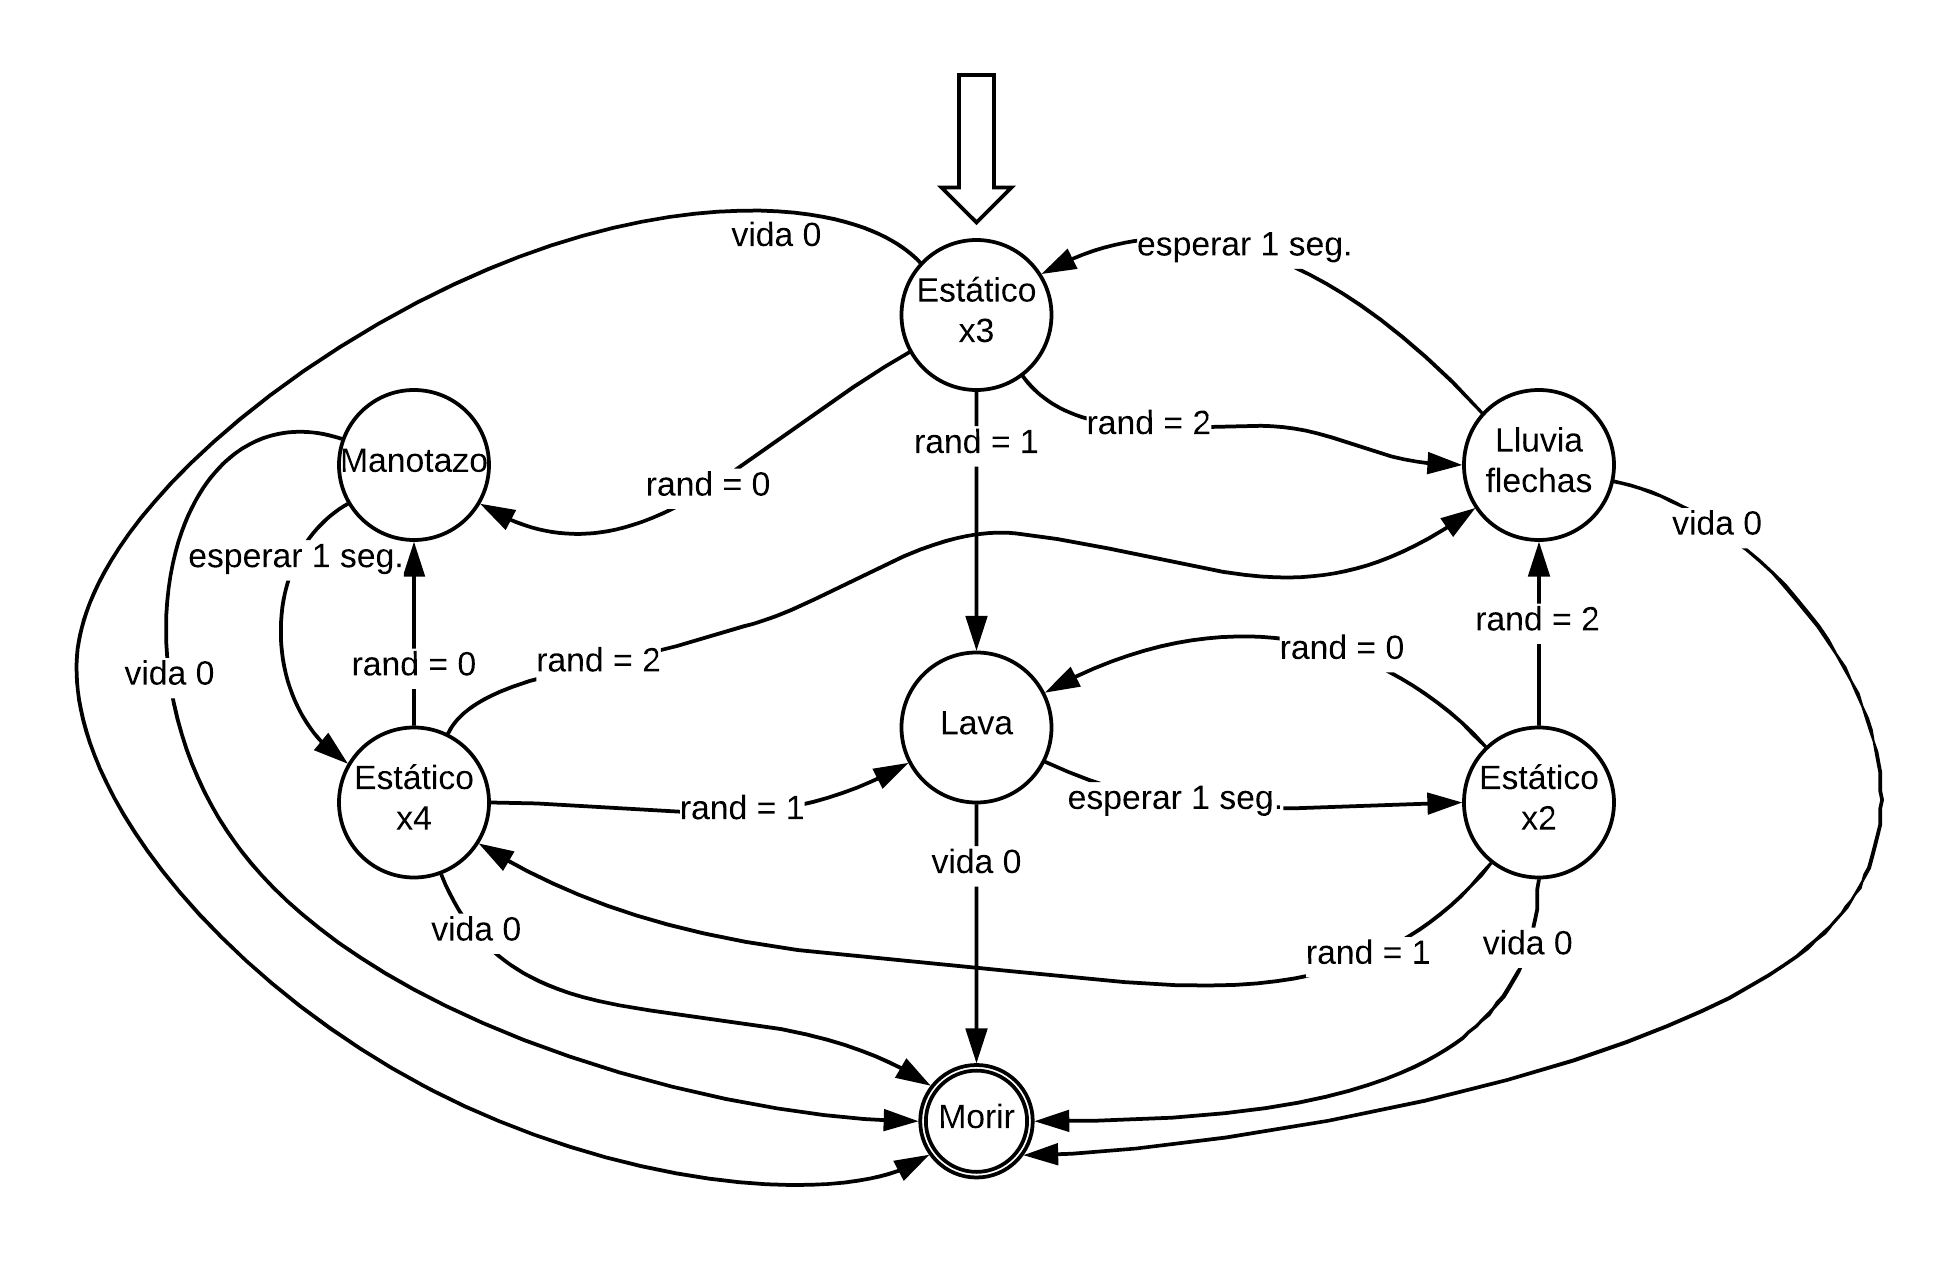
\includegraphics[width=0.5\textwidth]{imagenes\N7}
\end{figure}

\subsubsection{Jefe nivel 9}
Dada las acciones descritas anteriormente en el documento de diseño, se tiene estocada, filo y sablazo. Además se agregan otras acciones no contempladas para la ayuda de transiciones.
La nomenclatura queda como sigue:
\\[1pt]

\begin{itemize}
	\item Morir -> Mo
	\item Estocada -> Es
	\item Estático x4 -> Ex4 
	\item Sablazo -> Sa
	\item Filo -> Fi
	\item Jugador lejos -> Jl
	\item Rand 1 -> R1
	\item Rand 0 -> R0
	\item Vida 0 -> V0
	\item Esperar 1 seg. -> E1s
	\item Jugador cerca -> Jc
\end{itemize}
\\[1pt]

Los estados son:
\\[1pt]
Q = {Mo, Ex4, Es, Sa, Fi}
\\[1pt]

El alfabeto son:
\\[1pt]
\sigma = {Jl, Jc, E1s, R1, R0}
\\[1pt]

El estado inicio es:
\\[1pt]
q0 = {Ex4}
\\[1pt]

El estado final es:
\\[1pt]
F = {Mo}
\\[1pt]


Como vemos en la imagen \ref{fig:maqN9} queda representada la máquina de estados.
\begin{figure}
	\centering
	\caption{Máquina de estados que realiza el jefe del nivel 9}
	\label{fig:maqN9}
	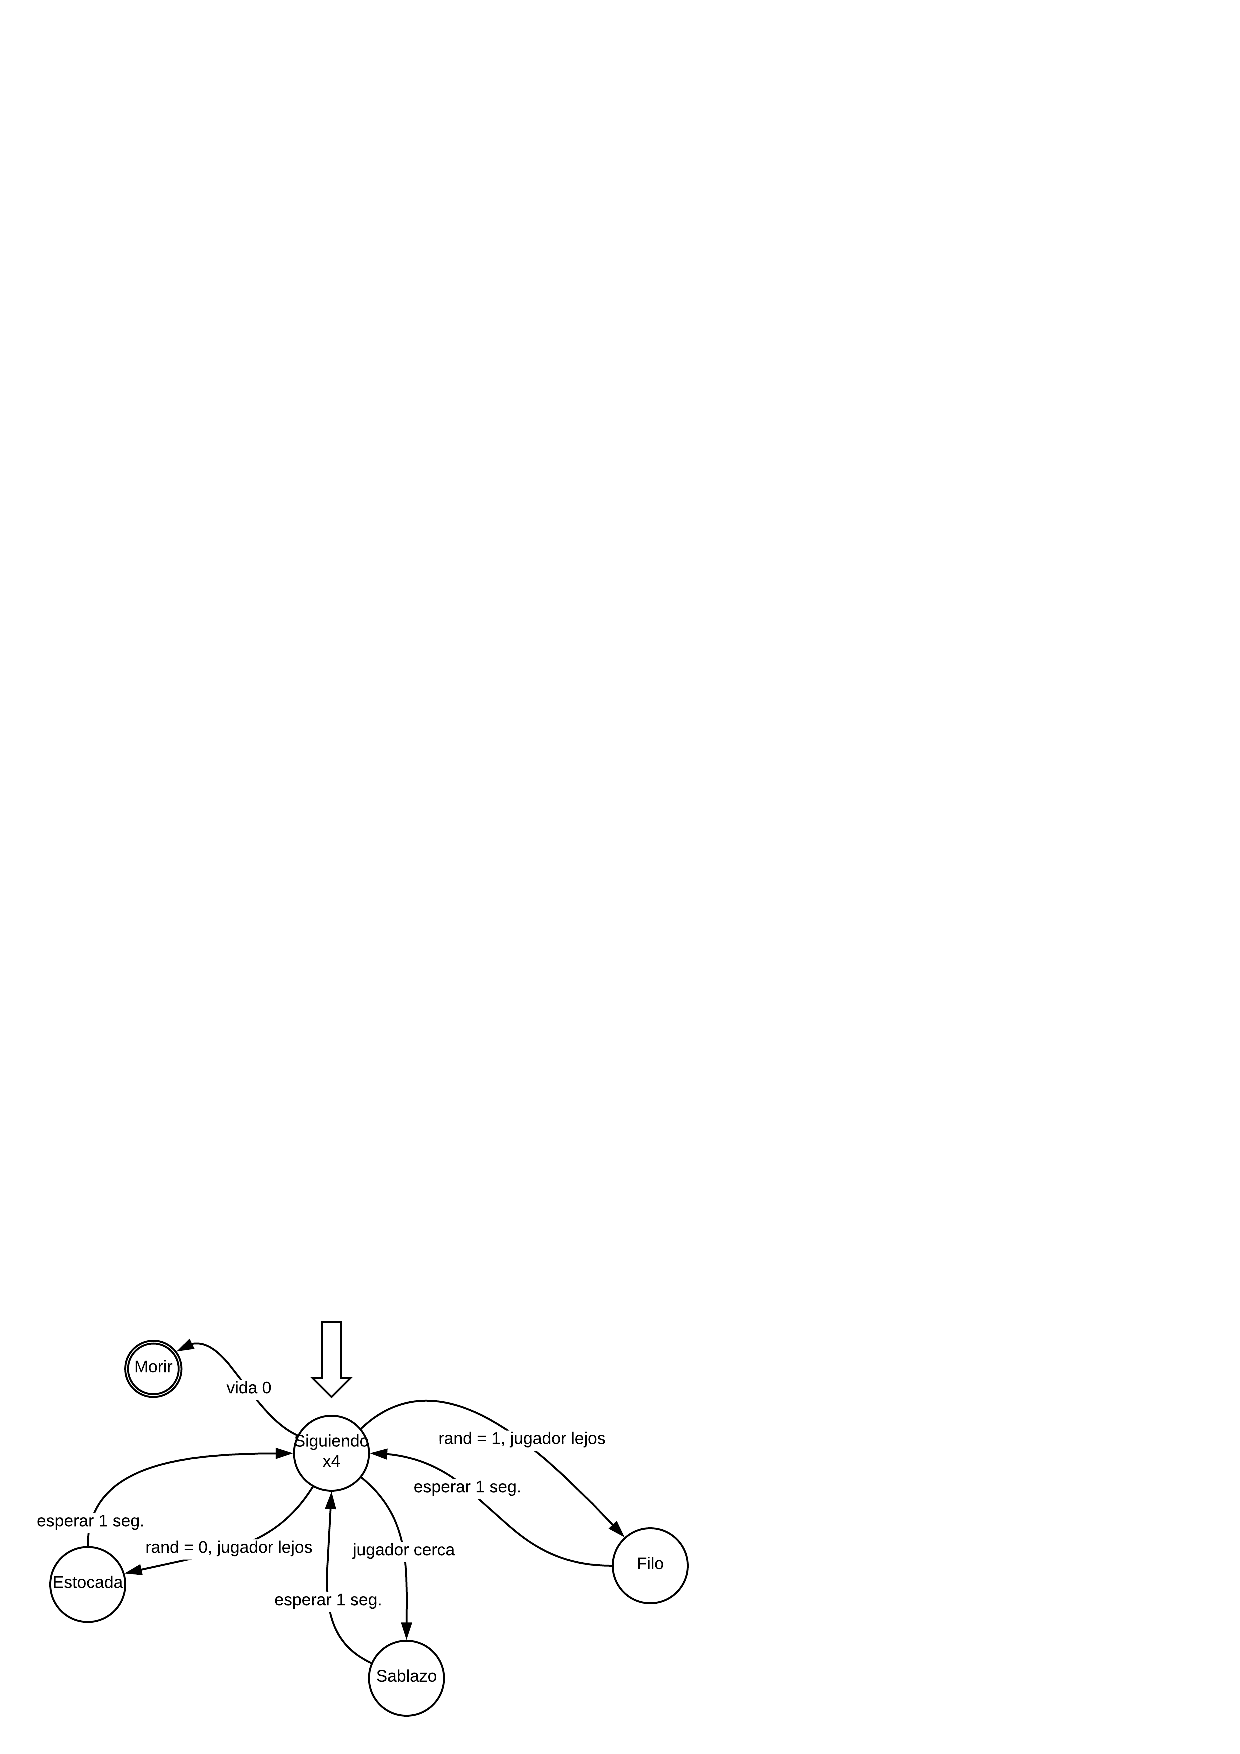
\includegraphics[width=0.5\textwidth]{imagenes\N9}
\end{figure}